Results are really satisfying given the fact that we knew absolutely none of the languages we used at the beginning and that the application is supposed to be a prototype. We ended up having more than 7000
lines of code in the languages described previously. There are still a few improvements to be made 
but for the moment one can import pictures from either his camera or his computer, sort them, delete them, launch a 3D recontruction on those images, and then see the result on the renderer and see cameras positions on a map.
We also implement interaction between the map and the photo list : if a user click on a picture, it will center the map on the GPS position of the camera used to take this picture. The user can also manage a workspace, even multiple workspaces, in which he can add scenes. One scene has one or multiple pictures, and it is from one scene that the user can launch a 3D reconstruction. The application comes with installation instructions and even a documentation (see ~\cite{doc}). To conclude on those results, we have, at the end of this project, a pretty good prototype and our clients were pretty satisfied with the result. Here is a screenshot of the application :
\begin{figure}[t]
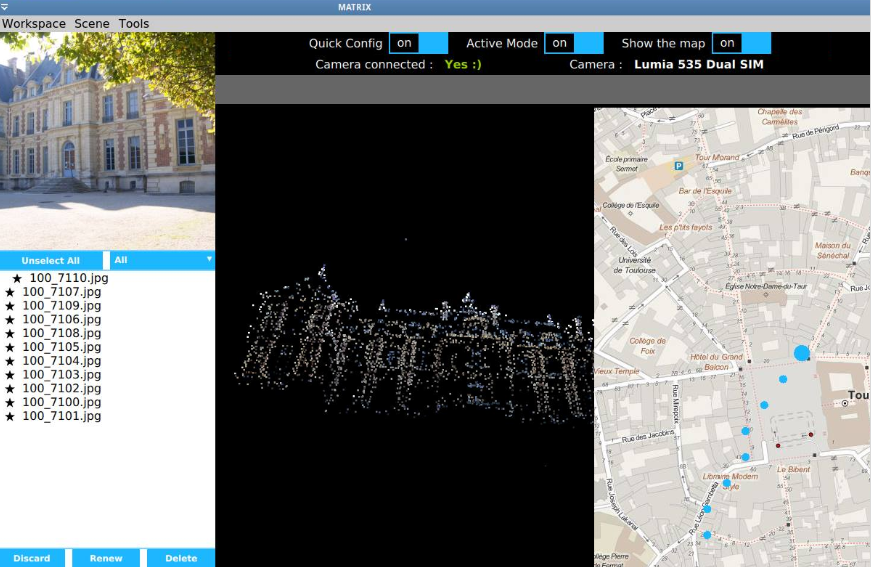
\includegraphics[width=\linewidth]{images/app.png}
\caption{Screenshot of the final application}
\label{app}
\vspace{-2mm}
\end{figure}

In further version, we could add the same type of interaction between the 3D renderer and the photo list. We could also launch the reconstruction in another thread to not block the entire application while a reconstruction is processed.